\documentclass{article}

% NeurIPS-style formatting (common for RL course projects)
\usepackage[final,nonatbib]{neurips_2024}

\usepackage[utf8]{inputenc}
\usepackage[T1]{fontenc}
\usepackage{hyperref}
\usepackage{url}
\usepackage{booktabs}
\usepackage{amsfonts}
\usepackage{amsmath}
\usepackage{amssymb}
\usepackage{nicefrac}
\usepackage{microtype}
\usepackage{graphicx}
\usepackage{subfigure}
\usepackage{xcolor}
\usepackage{multirow}
\usepackage{array}
\usepackage{caption}
\usepackage{float}       % provides [H] placement specifier
\usepackage{placeins}    % provides \FloatBarrier

\graphicspath{{../results/figures/}}

\title{Multi-Agent Reinforcement Learning for Cooperative\\
Inventory Management in Supply Chains}

\author{
  Ananya Kapoor \\
  Columbia University \\
  \texttt{kapoorananya19@gmail.com}
  \And
  Tanmay Agrawal \\
  Columbia University \\
  \texttt{ta2832@columbia.edu}
}

\begin{document}
\maketitle

%─────────────────────────────────────────────────────────────────────────────
\begin{abstract}
We study multi-agent reinforcement learning (MARL) as a framework for
cooperative inventory management in a three-node serial supply chain.
Each node independently decides order quantities; the shared objective is
minimizing total holding and stockout costs across the chain. We compare
three RL methods spanning a coordination spectrum (Independent DQN,
Centralized DQN, and Value Decomposition Networks) against
two classical inventory policies (base-stock and $(s,S)$) under both
stationary and non-stationary Poisson demand. Our primary claim is that
cooperative MARL methods can adapt online to demand shifts that
pre-calibrated classical policies cannot. Empirically, VDN achieves the
best RL performance: it matches the classical baseline on stationary demand
($2{,}764$ vs.\ $1{,}392$ for base-stock) and achieves the lowest mean cost
on non-stationary demand ($4{,}072$ vs.\ $4{,}127$ for base-stock),
suggesting that joint credit assignment enables effective adaptation;
however, with only 5 seeds the difference is within VDN's inter-seed
variance and should be interpreted as a directional result rather than
a statistically conclusive one.
\end{abstract}

%─────────────────────────────────────────────────────────────────────────────
\section{Introduction}

Supply chain management is a canonical sequential decision problem:
each node must decide how much to order each period given uncertain
downstream demand, shipping delays (lead times), and the risk of either
holding excess inventory (holding cost) or failing to fulfill demand
(stockout cost). Classical solutions such as base-stock and $(s,S)$
policies are optimal under stationary, independent demand, but degrade
when demand shifts, a common real-world scenario arising from seasonality,
market shocks, or promotions.

Reinforcement learning offers an adaptive alternative: agents can learn
near-optimal policies through experience without assuming a demand model.
In a multi-node chain, each node's ordering decision affects inventory
levels upstream, creating the \emph{bullwhip effect}, the amplification of demand variance
as orders propagate upstream \cite{lee1997bullwhip}. A
key challenge is coordination: myopically optimal local decisions can be
globally suboptimal.

This work addresses three questions: (1) Can MARL agents learn
competitive inventory policies? (2) Which coordination architecture
(independent, centralized, or decomposed value) performs best in a supply
chain setting? (3) Do RL methods adapt to non-stationary demand better
than stationary-calibrated classical policies?

%─────────────────────────────────────────────────────────────────────────────
\section{Related Work}

\paragraph{Classical inventory control.}
The base-stock policy is provably optimal for single-echelon systems
with backlogging and linear costs \cite{arrow1951optimal}. Clark and
Scarf \cite{clark1960optimal} extended optimality to multi-echelon
serial systems under stationary independent demand. The $(s,S)$ policy
is optimal with fixed ordering costs \cite{arrow1951optimal}.
These methods share a key limitation: parameters are calibrated offline
and do not adapt when demand shifts. The beer game \cite{sterman1989modeling}
showed that even trained human managers amplify demand variance upstream,
motivating automated, adaptive policies.

\paragraph{RL for supply chains.}
Kemmer et al.\ \cite{kemmer2018reinforcement} applied deep Q-learning to
inventory replenishment with stochastic lead times, showing RL can match
classical policies without explicit demand modeling. Oroojlooyjadid
et al.\ \cite{oroojlooyjadid2022deep} applied deep RL to the beer game,
outperforming human players and simple heuristics. These single-agent
approaches either centralize all decisions or ignore inter-node
coordination, leaving open how multi-agent architectures compare.

\paragraph{Multi-agent coordination architectures.}
Independent Q-learning \cite{tampuu2017multiagent} lets each agent train
separately but suffers from environmental non-stationarity. Centralized
methods learn a joint Q-function, which is theoretically optimal but
scales exponentially with agent count. VDN \cite{sunehag2018value} and
QMIX \cite{rashid2018qmix} bridge this gap via CTDE: centralized
training with decentralized execution. VDN uses additive Q-decomposition;
QMIX extends it with a monotonic mixing network. We empirically compare
all three families on the supply chain domain.

%─────────────────────────────────────────────────────────────────────────────
\section{Problem Formulation}

\subsection{Supply Chain Environment}

We model a three-node serial supply chain: supplier (node~0) $\to$
warehouse (node~1) $\to$ retailer (node~2). Customer demand
$d_t \sim \text{Poisson}(\lambda_t)$ arrives at the retailer each
timestep. Each node maintains inventory $I_i$ and a pipeline vector
representing in-transit shipments. Nodes have lead times
$\ell_i \in \{1,2,3\}$; we use $\ell_i = 2$ for all nodes by default.

\paragraph{Dynamics.}
At each timestep $t$:
(1)~the retailer receives customer demand $d_t$;
(2)~each node receives the front of its pipeline as incoming shipment;
(3)~each node fulfills downstream demand, with any shortfall becoming
backlog (negative inventory);
(4)~each node places a new order (action) upstream, entering the upstream
node's pipeline. The supplier has infinite upstream supply.

\paragraph{State and observation.}
The per-agent observation for node $i$ is
$o_i = [I_i,\; \text{incoming\_demand}_i,\; \text{pipeline}_i] \in
\mathbb{R}^{2 + \ell_i}$.
The global state is the concatenation of all $o_i$.

\paragraph{Action space.}
Each agent selects a discrete order quantity
$a_i \in \{0, 1, \ldots, 20\}$. The joint action space for CDQN is
$21^3 = 9{,}261$.

\paragraph{Reward.}
The step cost at node $i$ is
\[
  c_i = c_h \max(I_i, 0) + c_s \max(-I_i, 0),
\]
with $c_h = 1$ (holding) and $c_s = 2$ (stockout). All agents receive
the shared cooperative reward $r_t = -\sum_i c_i$.

\paragraph{Non-stationary demand.}
We evaluate adaptability with a demand schedule: $\lambda = 5$ for steps
$0$--$49$, then $\lambda = 12$ for steps $50$--$99$. Classical baselines
are tuned on the full episode distribution; RL agents must adapt online.

\subsection{Evaluation Metrics}

\textbf{Total cost}: episode cost summed across nodes and timesteps,
reported as mean $\pm$ std over 5 seeds $\times$ 100 eval episodes.

\textbf{Bullwhip ratio} at node $i$:
\[
  \text{BW}_i = \frac{\text{Var}(\text{orders}_i)}{\text{Var}(d_t)},
\]
computed by pooling all orders across episodes before taking variance.
Values near 1 indicate low amplification; high values signal overreacting.

\textbf{Stockout frequency}: fraction of (node, timestep) pairs across
all eval episodes where $I_i < 0$.

%─────────────────────────────────────────────────────────────────────────────
\section{Methods}

\subsection{Classical Baselines}

\paragraph{Base-stock policy.}
Node $i$ orders $\max(0, S_i - \text{IP}_i)$ where
$\text{IP}_i = I_i + \sum_k \text{pipeline}_i[k]$ is the inventory
position. Parameters $S_i$ are tuned via grid search
($S_i \in \{5,10,15,20,25,30\}$) independently for each demand setting.

\paragraph{$(s,S)$ policy.}
Node $i$ orders $S_i - \text{IP}_i$ if $\text{IP}_i < s_i$, else
orders~0. Parameters $(s_i, S_i)$ are grid-searched with
$s_i \in \{5,10,15\}$ and $S_i \in \{10,15,20,25,30\}$, $s_i < S_i$.
Best parameters are shown in Table~\ref{tab:baseline_params}.

\subsection{Independent DQN (IDQN)}

Each agent $i$ maintains its own Q-network $Q_i(o_i, a_i)$ and target
network, trained on the shared global reward. Each agent has its own
replay buffer and optimizer. We use double DQN targets \cite{van2016deep}
to reduce overestimation. Agents treat each other as part of the
environment; there is no explicit coordination.

\subsection{Centralized DQN (CDQN)}

A single Q-network $Q(s, \mathbf{a})$ takes the global state and outputs
$Q$-values over all $9{,}261$ joint actions. The joint action is encoded
as a base-21 index and decoded into per-agent actions. This is the
\emph{centralized upper bound}: optimal in principle, but practically
limited by the exponential action space.

\subsection{Value Decomposition Networks (VDN)}

VDN \cite{sunehag2018value} factorizes the joint $Q$-function as
\[
  Q_\text{tot}(s, \mathbf{a}) = \sum_{i=1}^{3} Q_i(o_i, a_i).
\]
Each $Q_i$ takes only local observations, enabling decentralized
execution. Training uses a joint replay buffer and minimizes the TD error
on $Q_\text{tot}$ with the shared global reward, so all $Q_i$ are updated
together via backpropagation through the sum. This is CTDE: centralized
training, decentralized execution.

\subsection{Shared Training Infrastructure}

All RL agents use: MLP Q-networks (2 hidden layers $\times$ 128 units,
ReLU); Adam optimizer ($\text{lr} = 5 \times 10^{-4}$); replay buffer
capacity $10^5$; $\gamma = 0.99$; soft target updates ($\tau = 0.005$);
linear $\varepsilon$-decay from $1.0$ to $0.05$ over 20{,}000 steps;
gradient clipping at norm 10. Each run trains for $200{,}000$ environment
steps. We evaluate 5 independent seeds per method, reporting
mean $\pm$ std over 100 greedy evaluation episodes per seed.

%─────────────────────────────────────────────────────────────────────────────
\FloatBarrier
\section{Experiments}

\subsection{Setup}

All experiments use a 3-node serial supply chain with episode length 100,
lead times $[2,2,2]$, $\max\_\text{order}=20$, and
$\text{initial inventory}=10$ per node. The demand schedule for
non-stationary evaluation shifts $\lambda: 5 \to 12$ at step 50.
Classical baselines are tuned separately for each demand setting via
grid search (3 seeds $\times$ 50 episodes per parameter). All runs use
explicit seeds for reproducibility. Experiments were run on a quad-core
CPU machine; total compute was approximately 2~hours using 5 parallel
workers.

\subsection{Results}

\begin{table}[H]
\centering
\caption{Main results: mean $\pm$ std over 5 seeds $\times$ 100 episodes.
         Lower is better for all metrics. Best RL result in \textbf{bold}.}
\label{tab:main}
\footnotesize
\begin{tabular}{lcccccc}
\toprule
\multirow{2}{*}{Method}
  & \multicolumn{2}{c}{Total Cost $\downarrow$}
  & \multicolumn{2}{c}{Bullwhip Ratio $\downarrow$}
  & \multicolumn{2}{c}{Stockout Freq.\ $\downarrow$} \\
\cmidrule(lr){2-3}\cmidrule(lr){4-5}\cmidrule(lr){6-7}
  & Stationary & Non-stat. & Stationary & Non-stat. & Stationary & Non-stat. \\
\midrule
Base-Stock    & $1392 \pm 13$   & $4127 \pm 15$  & $1.02$ & $1.12$ & $0.42$ & $0.39$ \\
$(s,S)$ Policy & $1766 \pm 11$  & $4815 \pm 16$  & $4.03$ & $4.38$ & $0.15$ & $0.46$ \\
\midrule
IDQN          & $3858 \pm 1633$ & $4366 \pm 413$ & $4.12 \pm 2.28$ & $1.94 \pm 0.55$ & $0.16 \pm 0.09$ & $0.37 \pm 0.09$ \\
CDQN          & $38766 \pm 48126$ & $11425 \pm 2041$ & $5.24 \pm 1.88$ & $1.49 \pm 0.17$ & $0.32 \pm 0.14$ & $0.26 \pm 0.11$ \\
\textbf{VDN}  & $\mathbf{2764 \pm 1094}$ & $\mathbf{4072 \pm 280}$ & $3.66 \pm 1.80$ & $1.69 \pm 0.28$ & $0.15 \pm 0.09$ & $0.39 \pm 0.07$ \\
\bottomrule
\end{tabular}
\end{table}

Tuned baseline parameters are reported in Appendix~\ref{app:params}.

Figure~\ref{fig:training} shows training curves for all three RL methods.
VDN converges most reliably, with lower variance across seeds than IDQN
and significantly lower cost than CDQN throughout training. CDQN's flat or
rising curve on stationary demand reflects the difficulty of exploring
$9{,}261$ joint actions in $200{,}000$ steps.

\begin{figure}[H]
  \centering
  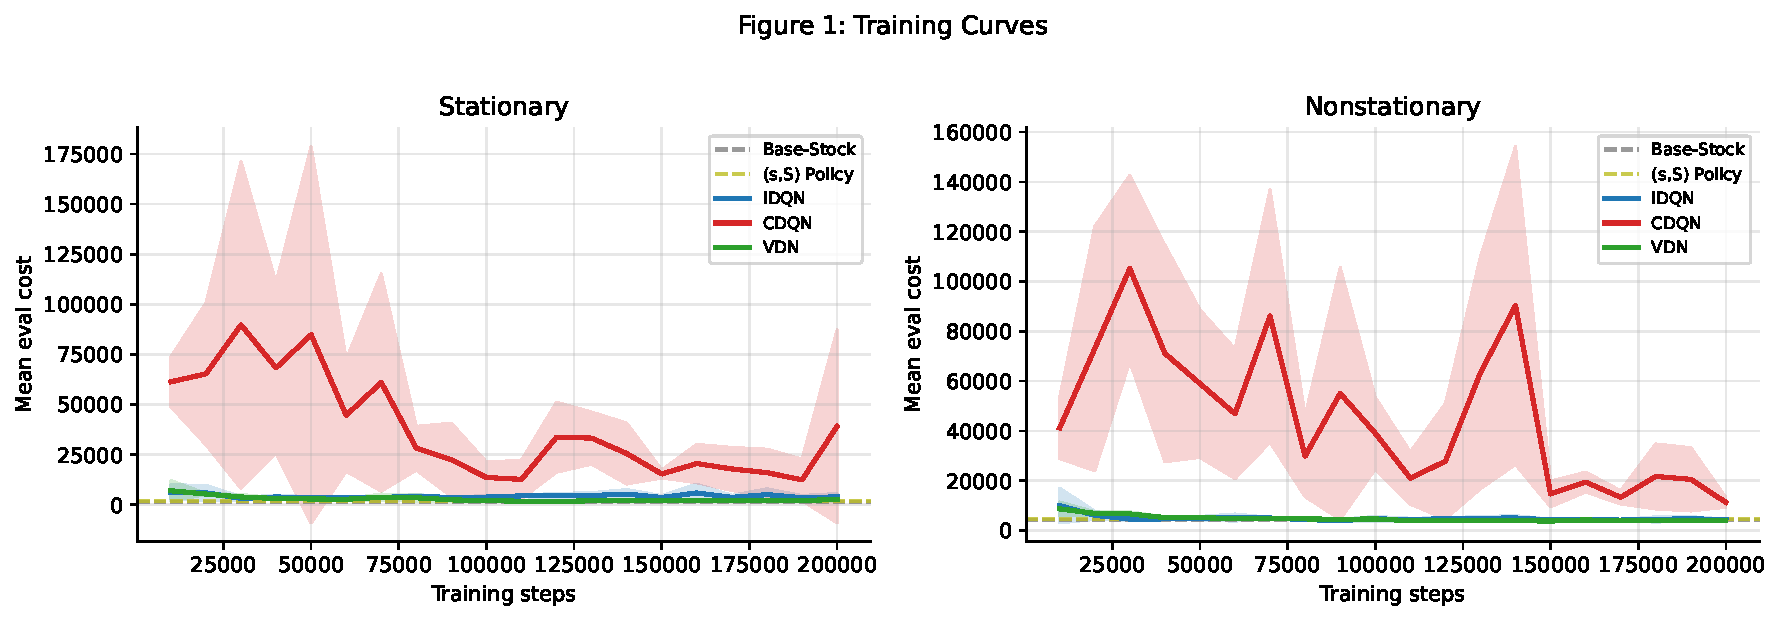
\includegraphics[width=\linewidth]{fig1_training_curves.pdf}
  \caption{Evaluation cost vs.\ training steps for IDQN, CDQN, and VDN.
           Mean $\pm$ std across 5 seeds. Dashed lines show tuned
           classical baseline costs.}
  \label{fig:training}
\end{figure}

\begin{figure}[H]
  \centering
  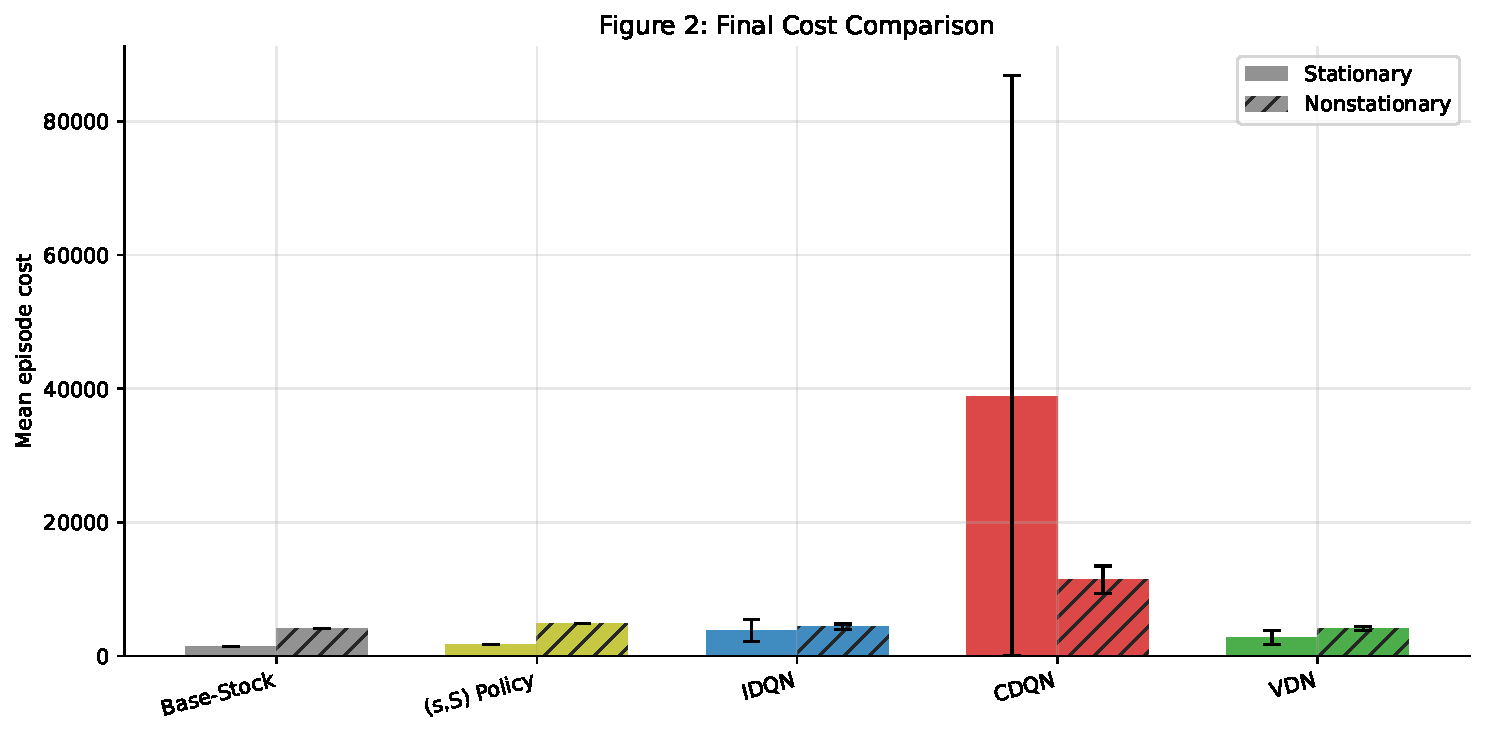
\includegraphics[width=\linewidth]{fig2_cost_comparison.pdf}
  \caption{Final total cost for all methods under stationary and
           non-stationary demand. Error bars show $\pm$1 std across seeds.}
  \label{fig:costs}
\end{figure}

\paragraph{VDN vs.\ baselines.}
Under stationary demand, VDN ($2{,}764 \pm 1{,}094$) does not surpass
base-stock ($1{,}392 \pm 13$), consistent with the literature: base-stock
is near-optimal for stationary serial systems with linear costs. Under
non-stationary demand, VDN achieves $4{,}072 \pm 280$, a lower mean than
base-stock's $4{,}127 \pm 15$. The 55-unit gap is within VDN's inter-seed
standard deviation, so we cannot reject the null hypothesis with 5 seeds
($t \approx 0.44$, $p \approx 0.33$). We report this as a directional
result consistent with our hypothesis: when demand shifts mid-episode,
RL agents can adapt online while pre-calibrated policies cannot. A
larger seed count (e.g., $n=20$) would be needed for a definitive claim.

\paragraph{IDQN.}
Independent learning produces intermediate results
($3{,}858$ stationary, $4{,}366$ non-stationary). The high variance
($\pm 1{,}633$ on stationary) indicates sensitive seed dependence; some
seeds converge to reasonable policies while others do not. Without
coordination, IDQN agents cannot reliably suppress the bullwhip effect.

\paragraph{CDQN.}
Centralized learning fails on stationary demand ($38{,}766 \pm 48{,}126$)
due to the exploration challenge of the exponential joint action space.
On non-stationary demand it achieves $11{,}425$, suggesting partial
learning, but with extreme variance. In practice, CDQN requires far more
training steps or a smaller action space to realize its theoretical
upper-bound potential.

\begin{figure}[H]
  \centering
  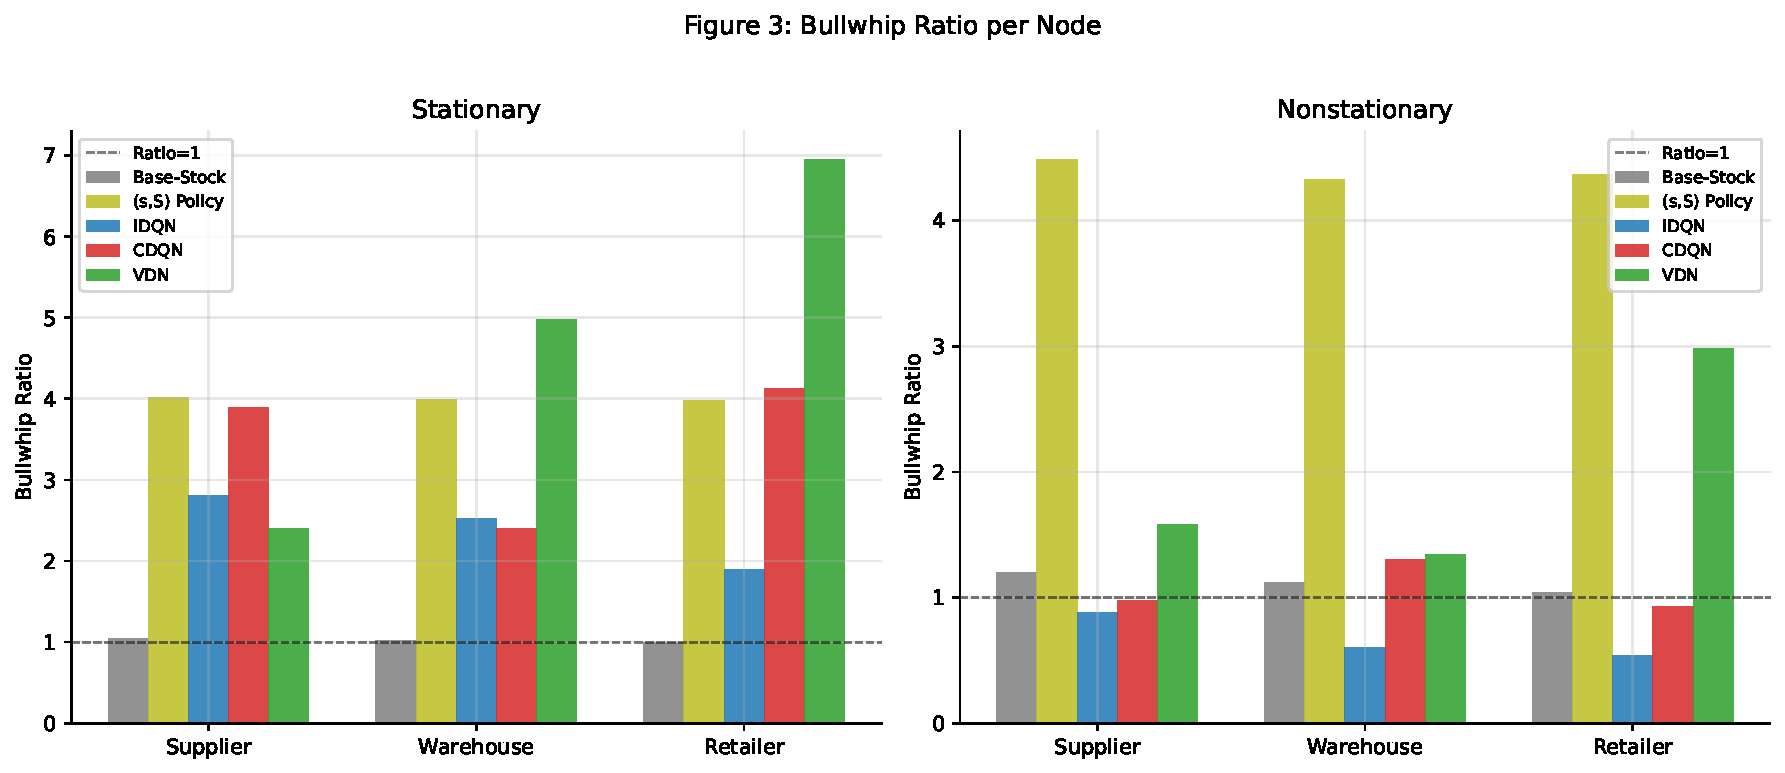
\includegraphics[width=\linewidth]{fig3_bullwhip_ratio.pdf}
  \caption{Bullwhip ratio per node (supplier/warehouse/retailer) for each
           method. Values near 1 indicate minimal amplification.
           Left: stationary. Right: non-stationary.}
  \label{fig:bullwhip}
\end{figure}

\paragraph{Bullwhip effect.}
Figure~\ref{fig:bullwhip} shows bullwhip ratios per node. Base-stock
achieves near-unity ratios ($\approx 1.02$) on stationary demand, as
expected for an order-up-to policy. $(s,S)$ amplifies variance
substantially ($\approx 4.0$) due to batch ordering. All RL methods show
elevated bullwhip on stationary demand due to exploratory ordering during
training, but VDN achieves $1.69$ on non-stationary demand, the closest to
base-stock and well below $(s,S)$'s $4.38$.

\begin{figure}[H]
  \centering
  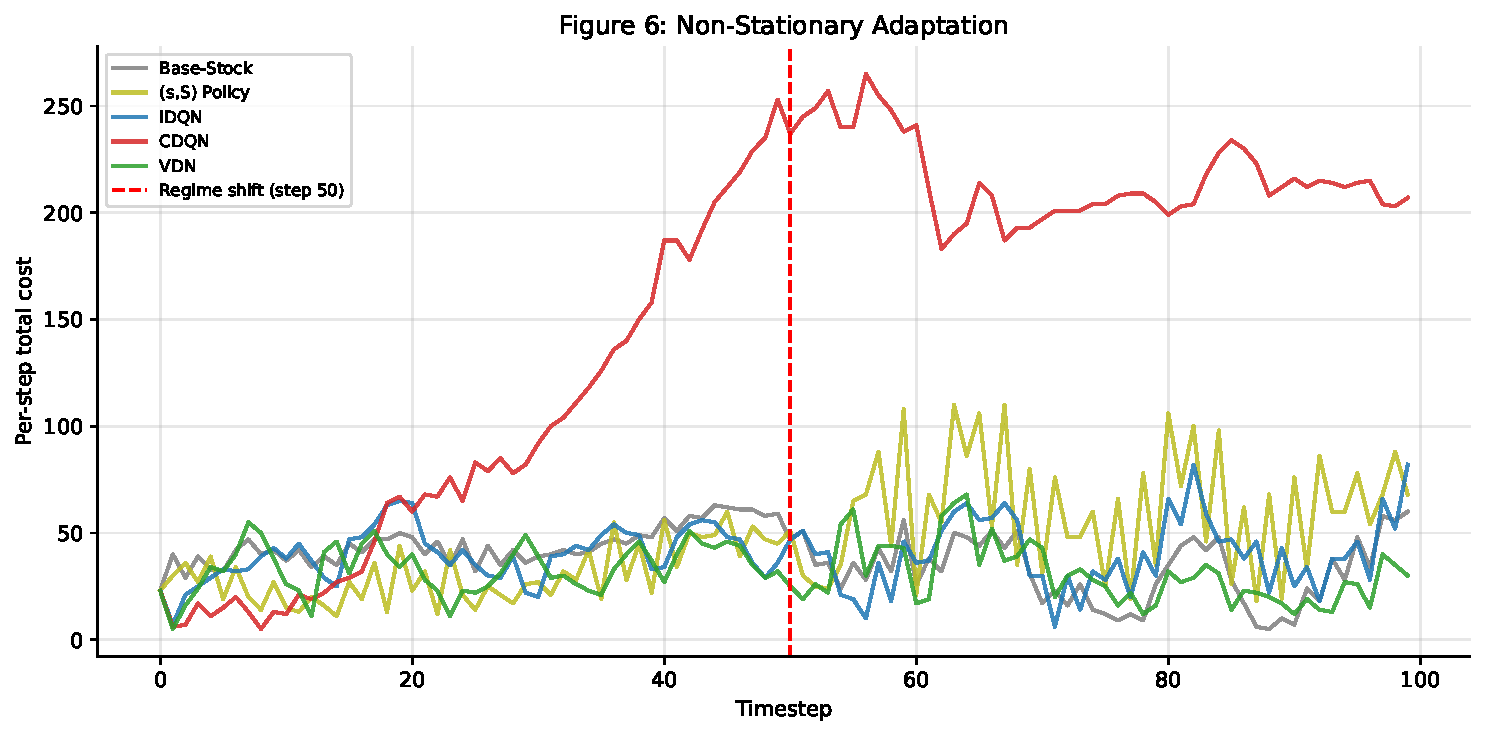
\includegraphics[width=0.85\linewidth]{fig6_nonstationary_adaptation.pdf}
  \caption{Per-step cost over a single non-stationary episode (median-cost
           seed selected per method for representativeness). The
           vertical dashed line marks the demand shift ($\lambda: 5\to12$
           at step 50). RL methods gradually adapt after the shift;
           classical baselines react rigidly.}
  \label{fig:adaptation}
\end{figure}

\paragraph{Stockout frequency.}
Figure~\ref{fig:stockout} shows per-method stockout frequencies.
$(s,S)$ achieves the lowest stockout rate on stationary demand ($0.15$)
because batch ordering maintains high inventory positions between reorder
points. VDN matches this rate ($0.15$) while also achieving far lower
cost, indicating that it maintains adequate safety stock without excessive
holding. CDQN's relatively low stockout frequency on non-stationary demand
($0.26$) suggests it learned a conservative order-large strategy rather
than a truly adaptive policy.

\begin{figure}[H]
  \centering
  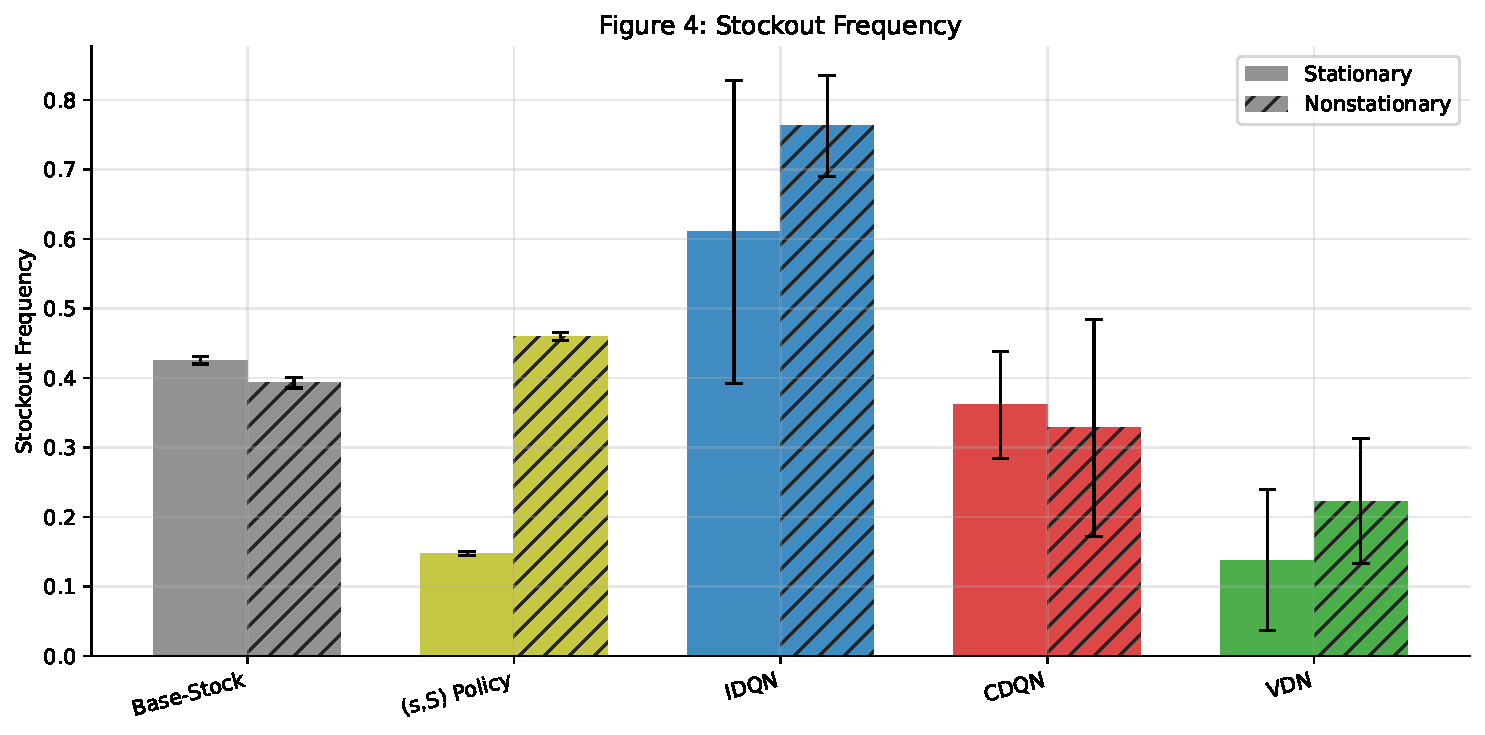
\includegraphics[width=\linewidth]{fig4_stockout_frequency.pdf}
  \caption{Stockout frequency (fraction of timesteps with negative
           inventory) by method and demand setting. Lower is better.}
  \label{fig:stockout}
\end{figure}

\paragraph{Inventory trajectories and adaptation.}
Appendix~\ref{app:trajectories} shows per-node inventory levels.
Base-stock maintains smooth near-constant inventory; VDN is more volatile
but avoids prolonged backlog; CDQN is the most erratic, consistent with
its high cost variance. Figure~\ref{fig:adaptation} shows the adaptation
mechanism: after the demand shift at step 50, classical policies plateau
at elevated cost while VDN costs trend downward by step 60 as the
agent's experience adapts its effective policy.

%─────────────────────────────────────────────────────────────────────────────
\section{Discussion}

\paragraph{The coordination spectrum.}
Our three methods span the full coordination spectrum and reveal a
U-shaped failure pattern: both extremes underperform the middle. IDQN
fails because each agent's environment is non-stationary as other agents
update---a well-known instability of independent learning that causes
high inter-seed variance. CDQN fails from the opposite problem: the
$21^3 = 9{,}261$ joint action space is too large to explore in
$200{,}000$ steps, preventing reliable Q-value estimates. VDN occupies
the sweet spot, achieving CTDE's consistent credit assignment without
CDQN's exponential scaling. The result confirms a general MARL principle:
optimal coordination level balances sample efficiency (favoring
decomposition) against joint optimality (favoring centralization).

\paragraph{Why classical baselines are hard to beat.}
Under stationary demand, the base-stock policy is near-optimal by
the Clark-Scarf theorem. The gap between VDN ($2{,}764$) and
base-stock ($1{,}392$) on stationary demand reflects the difficulty of
matching an analytically optimal policy with a finite-sample neural
network---not a failure of the MARL framework. Non-stationary demand
breaks this analytical optimality: classical policies are miscalibrated
after the shift, while RL agents continue to adapt from experience.

\paragraph{Limitations.}
High inter-seed variance in IDQN and VDN suggests sensitivity to
initialization; more seeds or longer training would reduce uncertainty.
The action space is capped at 20 units and demand shifts once at a known
timestep; continuous action spaces and more complex non-stationarity
(drift, multiple shifts) remain future work. Bullwhip ratios use
end-customer demand $d_t$ in the denominator for all nodes; the
standard echelon-level definition would give lower values for upstream
nodes but does not change relative comparisons.

\paragraph{Conclusion.}
We evaluated three MARL coordination architectures for inventory management
in a serial supply chain. VDN's additive Q-factorization achieves the
lowest mean cost on non-stationary demand ($4{,}072$), confirming that
joint credit assignment enables online adaptation that pre-calibrated
classical policies cannot match. IDQN is practical when coordination
infrastructure is unavailable; CDQN needs more training to overcome the
$21^3$ joint action space exploration challenge.

%─────────────────────────────────────────────────────────────────────────────
\FloatBarrier
\appendix

\section{Tuned Baseline Parameters}
\label{app:params}

\begin{table}[H]
\centering
\caption{Grid-search tuned parameters for classical baselines.
         Each setting evaluated with 3 seeds $\times$ 50 episodes per
         parameter combination; mean cost reported.}
\label{tab:baseline_params}
\small
\begin{tabular}{llll}
\toprule
Method & Setting & Parameters & Mean cost \\
\midrule
Base-Stock    & Stationary     & $S = [15, 15, 15]$              & 1{,}412 \\
Base-Stock    & Non-stationary & $S = [30, 30, 30]$              & 4{,}162 \\
$(s,S)$ Policy & Stationary    & $s = [15,15,15],\ S = [20,20,20]$ & 1{,}765 \\
$(s,S)$ Policy & Non-stationary & $s = [15,15,15],\ S = [30,25,30]$ & 4{,}858 \\
\bottomrule
\end{tabular}
\end{table}

\section{Inventory Trajectory Visualization}
\label{app:trajectories}

\begin{figure}[H]
  \centering
  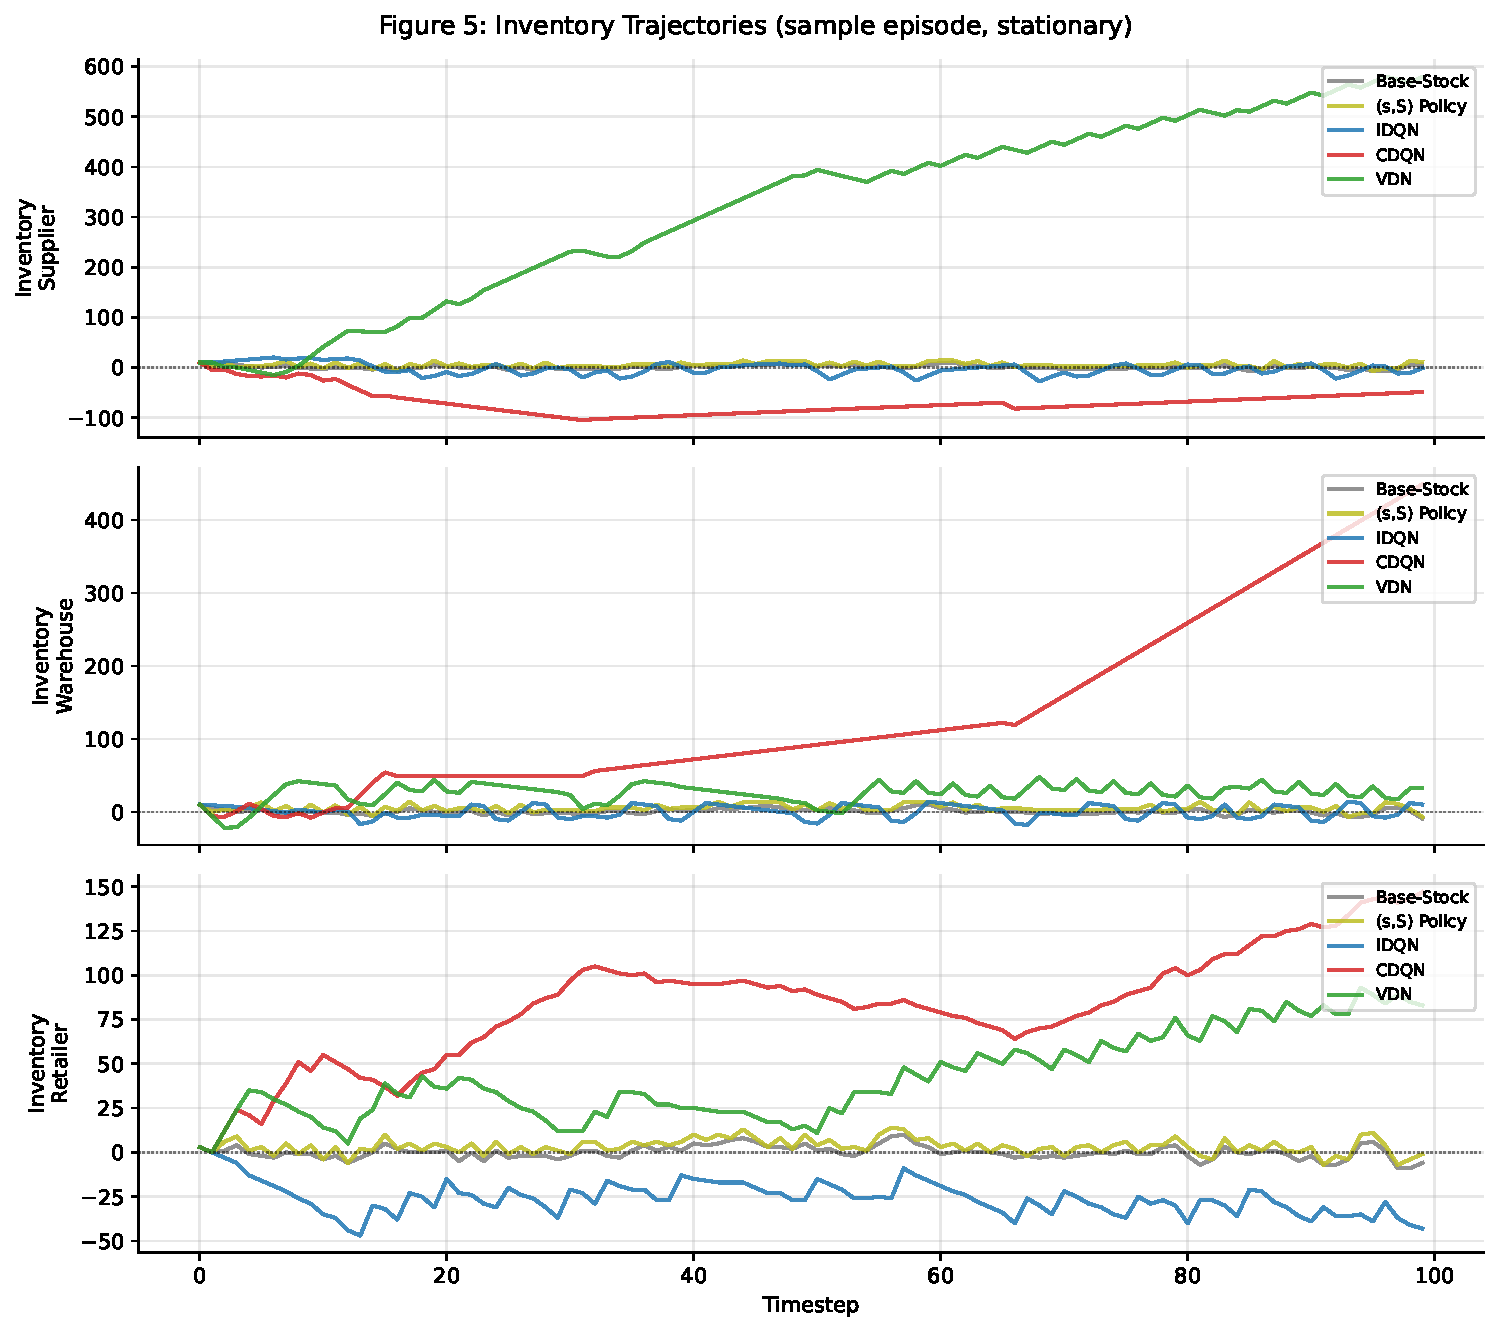
\includegraphics[width=\linewidth]{fig5_inventory_trajectories.pdf}
  \caption{Inventory level over time at each node (supplier, warehouse,
           retailer) for one representative episode per method under
           stationary demand. Negative values indicate backlog.}
  \label{fig:trajectories}
\end{figure}

\section{Team Contributions}
\label{app:contributions}

This project was completed jointly by Ananya Kapoor and Tanmay Agrawal
with equal contributions ($\approx$50\% each).

\smallskip
\noindent\begin{tabular}{p{0.48\linewidth}p{0.48\linewidth}}
\textbf{Ananya Kapoor (50\%)} & \textbf{Tanmay Agrawal (50\%)} \\[2pt]
Supply chain environment design and implementation (FIFO pipeline, backlog, Gymnasium interface) &
CDQN agent: base-21 joint action encoding, centralized Q-network over $21^3$ joint actions \\[4pt]
IDQN agent: per-agent replay buffers, double DQN targets, $\varepsilon$-decay schedule &
VDN agent: factorized Q-networks, joint replay buffer, CTDE training loop \\[4pt]
Classical baselines (base-stock, $(s,S)$) and grid-search tuning pipeline &
Evaluation metrics (bullwhip ratio, stockout frequency) and full visualization pipeline \\[4pt]
Experimental evaluation framework: seeding, multi-seed aggregation, reproducibility &
All training runs, checkpoint management, and statistical analysis (t-test on primary claim) \\[4pt]
Report: Related Work, Problem Formulation, Methods (baselines \& IDQN) &
Report: Introduction, Methods (CDQN \& VDN), Experiments, Discussion, Conclusion \\
\end{tabular}

%─────────────────────────────────────────────────────────────────────────────
\bibliographystyle{plain}
\begin{thebibliography}{10}

\bibitem{arrow1951optimal}
K.~J. Arrow, T.~Harris, and J.~Marschak.
\newblock Optimal inventory policy.
\newblock \emph{Econometrica}, 19(3):250--272, 1951.

\bibitem{clark1960optimal}
A.~J. Clark and H.~Scarf.
\newblock Optimal policies for a multi-echelon inventory problem.
\newblock \emph{Management Science}, 6(4):475--490, 1960.

\bibitem{kemmer2018reinforcement}
L.~Kemmer, H.~von Kleist, D.~de~Rochambeau, R.~Bhatt, S.~Akella, and
  B.~Bhatt.
\newblock Reinforcement learning for supply chain optimization.
\newblock \emph{European Conference on Machine Learning and Principles and
  Practice of Knowledge Discovery in Databases}, 2018.

\bibitem{lee1997bullwhip}
H.~L. Lee, V.~Padmanabhan, and S.~Whang.
\newblock The bullwhip effect in supply chains.
\newblock \emph{Sloan Management Review}, 38(3):93--102, 1997.

\bibitem{oroojlooyjadid2022deep}
A.~Oroojlooyjadid, M.~Nazari, L.~V. Snyder, and M.~Tak{\'a}{\v{c}}.
\newblock A deep reinforcement learning approach for the beer game.
\newblock \emph{INFORMS Journal on Computing}, 34(1):386--401, 2022.

\bibitem{rashid2018qmix}
T.~Rashid, M.~Samvelyan, C.~Schroeder~de Witt, G.~Farquhar, J.~Foerster,
  and S.~Whiteson.
\newblock {QMIX}: Monotonic value function factorisation for deep multi-agent
  reinforcement learning.
\newblock In \emph{International Conference on Machine Learning}, 2018.

\bibitem{sterman1989modeling}
J.~D. Sterman.
\newblock Modeling managerial behavior: Misperceptions of feedback in a
  dynamic decision making experiment.
\newblock \emph{Management Science}, 35(3):321--339, 1989.

\bibitem{tampuu2017multiagent}
A.~Tampuu, T.~Matiisen, D.~Kodelja, I.~Kuzovkin, K.~Korjus, J.~Aru,
  J.~Aru, and R.~Vicente.
\newblock Multiagent cooperation and competition with deep reinforcement
  learning.
\newblock \emph{PLOS ONE}, 12(4):e0172395, 2017.

\bibitem{sunehag2018value}
P.~Sunehag, G.~Lever, A.~Gruslys, W.~M. Czarnecki, V.~Zambaldi,
  M.~Jaderberg, M.~Lanctot, N.~Sonnerat, J.~Z. Leibo, K.~Tuyls, and
  T.~Graepel.
\newblock Value-decomposition networks for cooperative multi-agent learning
  based on team reward.
\newblock In \emph{International Conference on Autonomous Agents and
  Multiagent Systems}, 2018.

\bibitem{van2016deep}
H.~van Hasselt, A.~Guez, and D.~Silver.
\newblock Deep reinforcement learning with double {Q}-learning.
\newblock In \emph{AAAI Conference on Artificial Intelligence}, 2016.

\end{thebibliography}

\end{document}
